\chapter{CT Convolution}

\section{Review CT LTI systems and superposition property}

Recall the superposition property of LTI systems. If a CT system is LTI then the superposition property holds. Given a system where
\[   
x_i(t) \mapsto y_i(t) \; \forall\; i
\]
then
\[
\sum\limits_{i} a_i x_i(t) \mapsto \sum\limits_{i} a_i y_i(t) 
\]

Superposition enables a powerful problem reduction strategy. The overall idea for is that if:

\begin{itemize}
\item we can write an arbitrary signal as a sum of simple signals, and 
\item we can determine the response to the simple signals, then
\item we can easily express the output due to the input using superposition
\end{itemize}

This will be a recurring pattern in this course. In this lecture, the simple signals are weighted, time shifts of one signal, the delta function, $\delta(t)$.

\section{Convolution Integral}

To derive this we start with the sifting property of the CT impulse function (from chapter 2)
\[
\int\limits_{a}^{b} x(t)\delta(t-t_0) \; dt = x(t_0)
\]
for any $a < t_0 < b$. A slight change of variables ($t_0 \rightarrow \tau$) and limits ($a \rightarrow -\infty$ and $b \rightarrow \infty$) gives:
\[
x(t) = \int\limits_{-\infty}^{\infty} x(\tau)\delta(t-\tau) \; d\tau
\]
showing that we can write any CT signal as an infinite sum (integral) of weighted and time-shifted impluse functions.

Let $h(t)$ be the CT {\it impulse response}, the output due to the input $\delta(t)$, i.e. $\delta(t) \mapsto h(t)$. Then if the system is time-invariant: $\delta(t-\tau) \mapsto h(t-\tau)$ and by superposition if the input is writen as
\[
x(t) = \int\limits_{-\infty}^{\infty} x(\tau)\delta(t-\tau) \; d\tau
\]
then the output is given by
\[
  y(t) = \int\limits_{-\infty}^{\infty} x(\tau)h(t-\tau) \; d\tau = x(t) * h(t)
\]
This is called the \emph{convolution integral} \index{CT Convolution}.

It is worth pausing here to see the signifigance. For a LTI CT system, if I know its impulse response $h(t)$, I can find the response due to \textbf{any} input using convolution. For this reason the impulse response is another way to represent an LTI system.

\section{Graphical View of the Convolution Integral.}

Let us break the convolution expression down into pieces. In its general form the convolution of two signals $x_1(t)$ and $x_2(t)$ is
\[
x_1(t) * x_2(t) = \int\limits_{-\infty}^{\infty} x_1(\tau)x_2(t-\tau) \; d\tau
\]

Suppose $x_1(t)$ and $x_2(t)$ are signals that look like
\begin{center}
  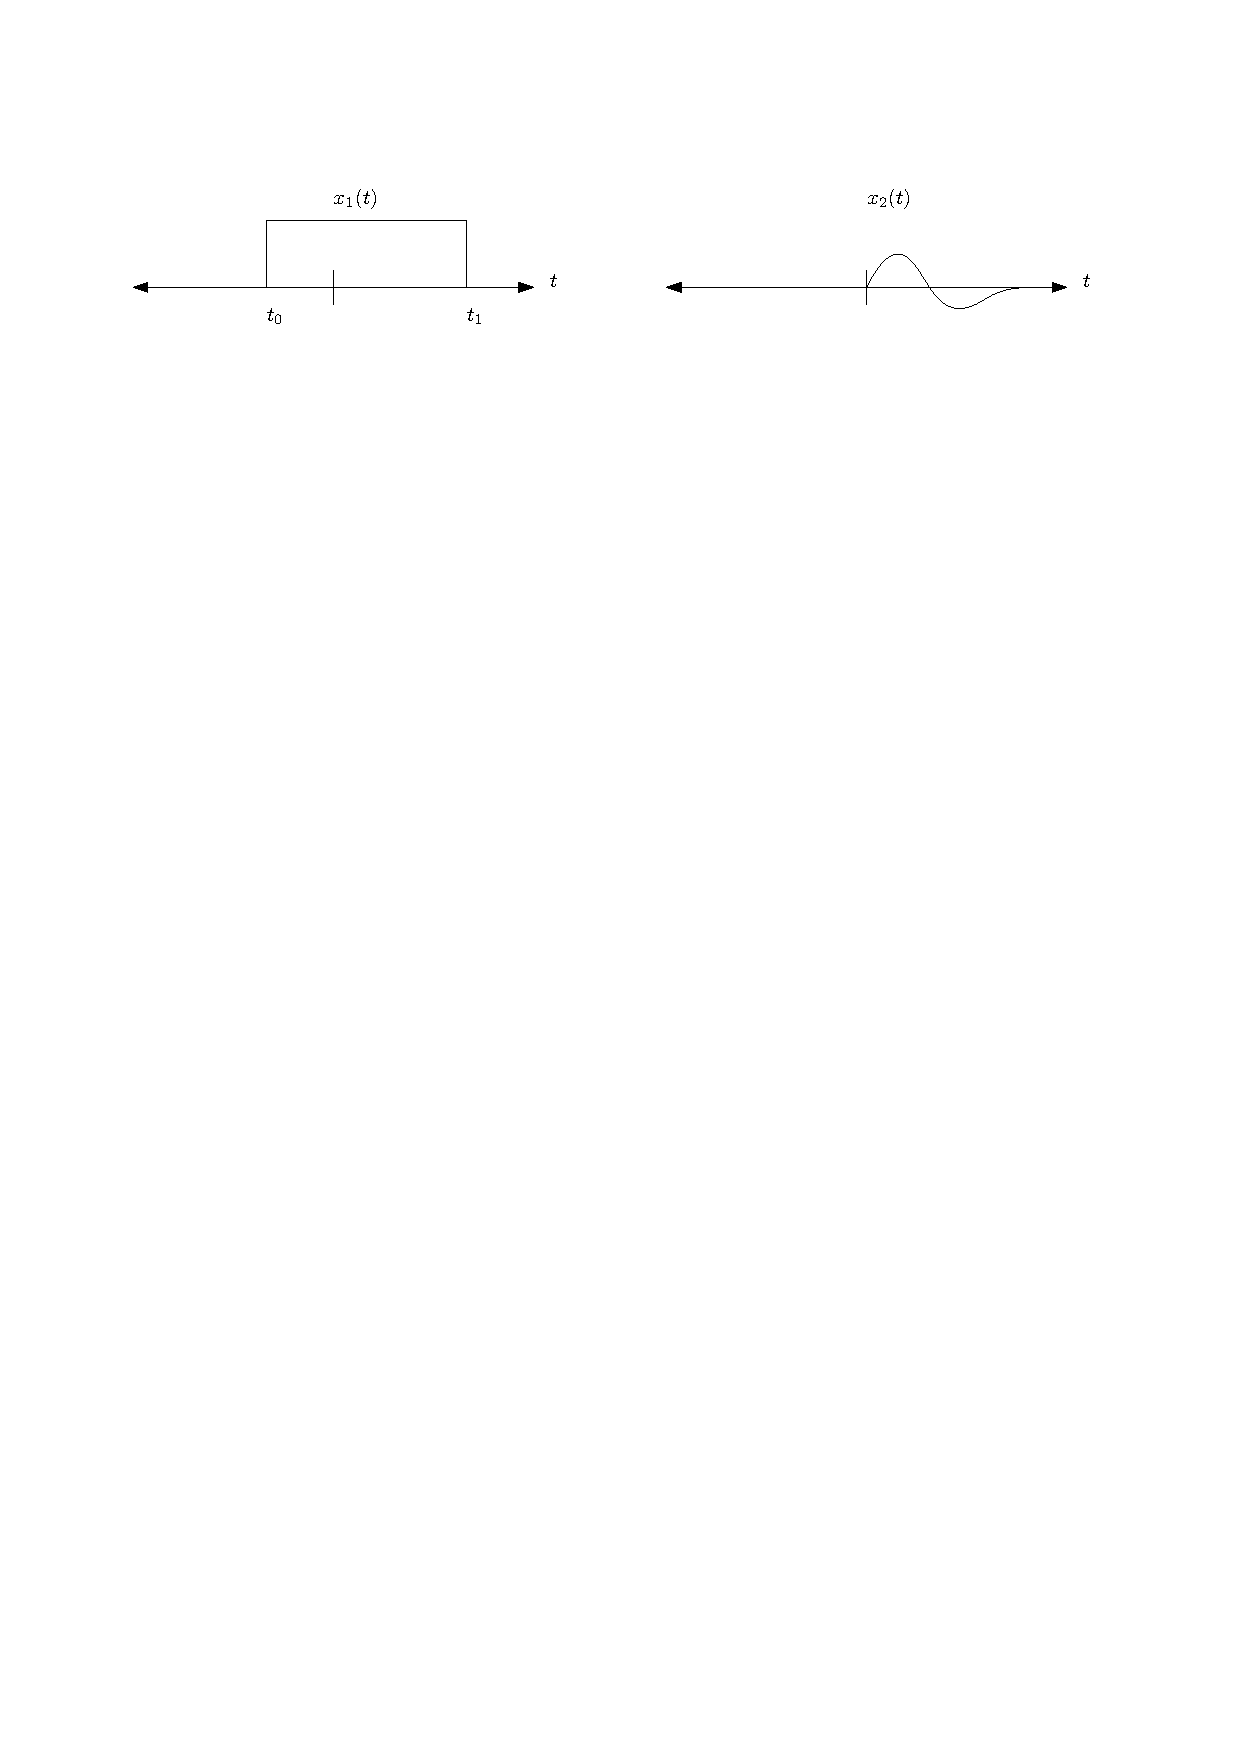
\includegraphics[scale=1]{graphics/convolution-explain1.pdf}
\end{center}

Then $x_1(\tau)$ and $x_2(-\tau)$ look like
\begin{center}
  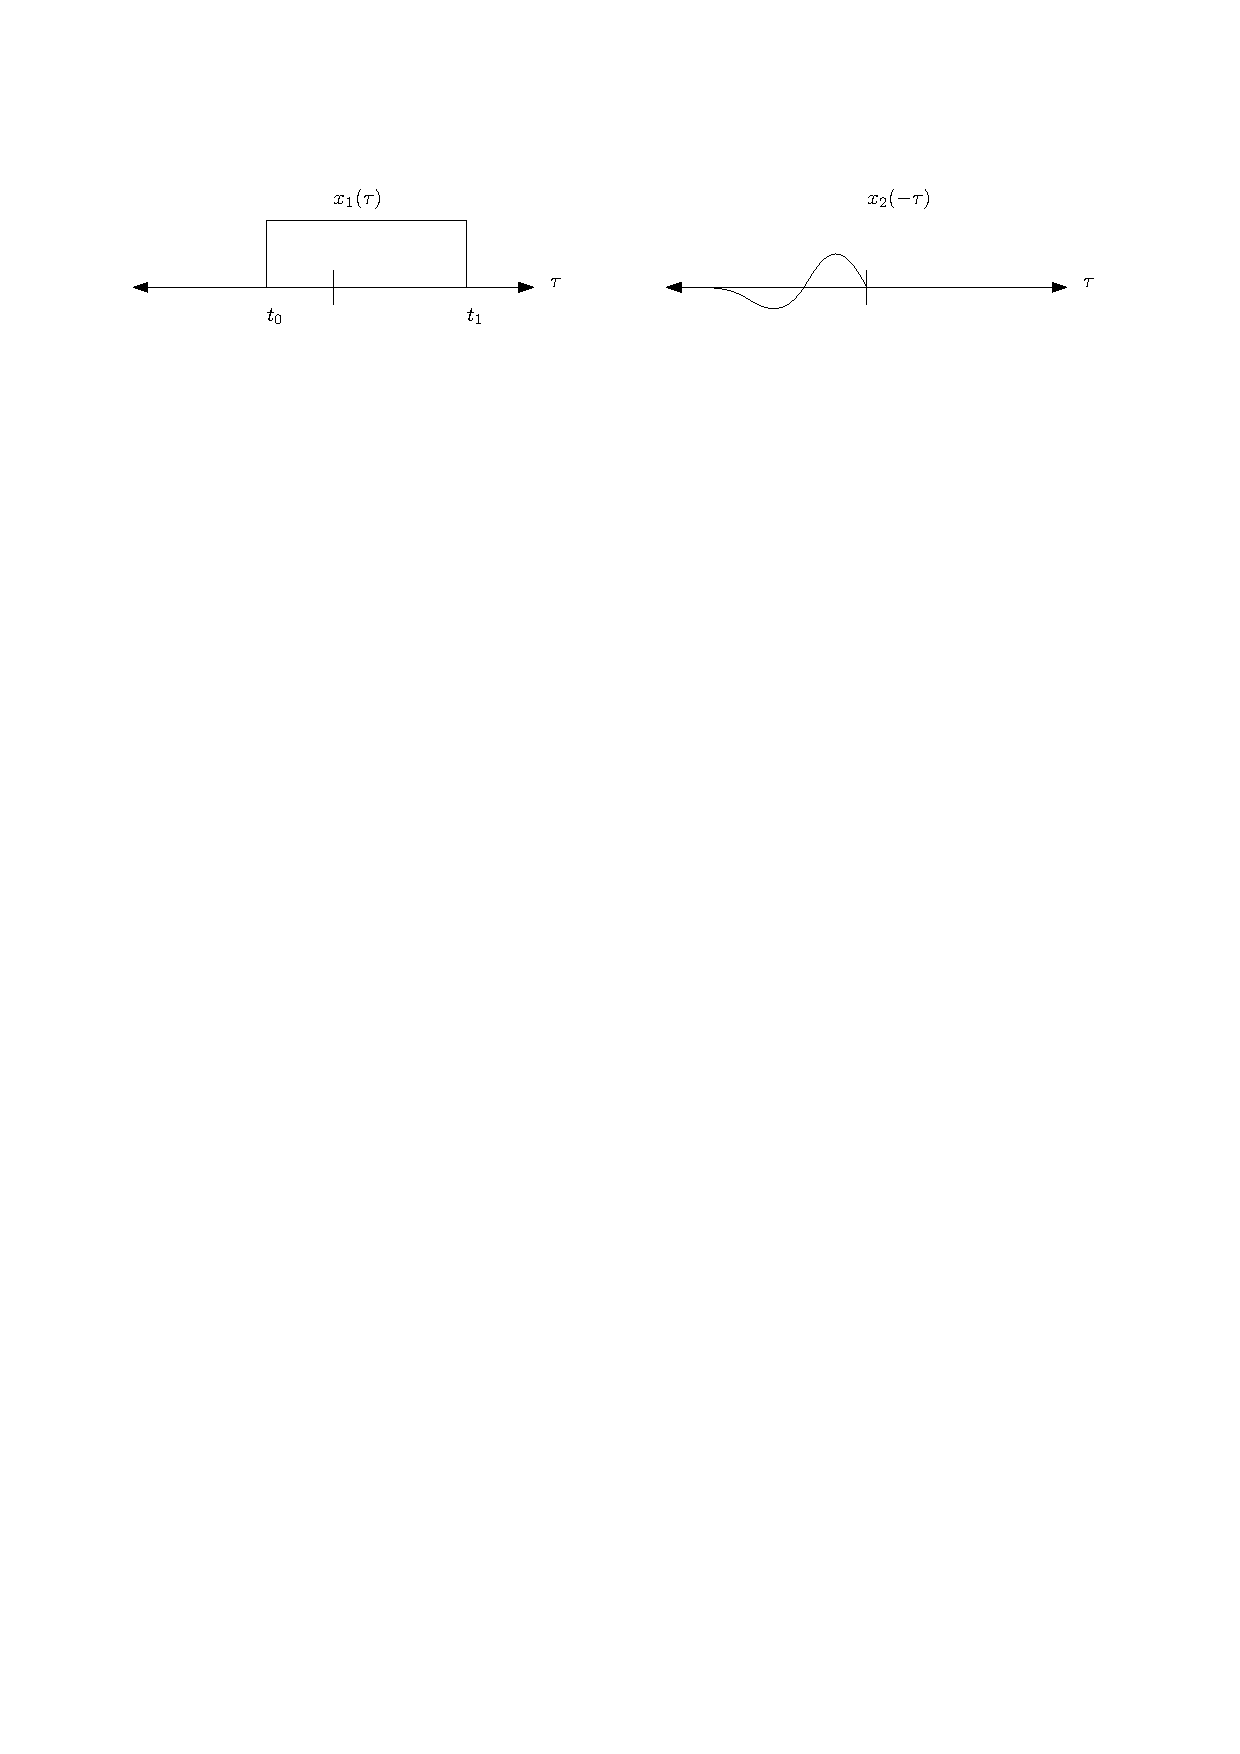
\includegraphics[scale=1]{graphics/convolution-explain2.pdf}
\end{center}
The signal $x_2(t-\tau)$ is $x_2(-\tau)$ shifted by $t$ (since $x_2(-\tau+t)= x_2(t-\tau)$) and then looks like
\begin{center}
  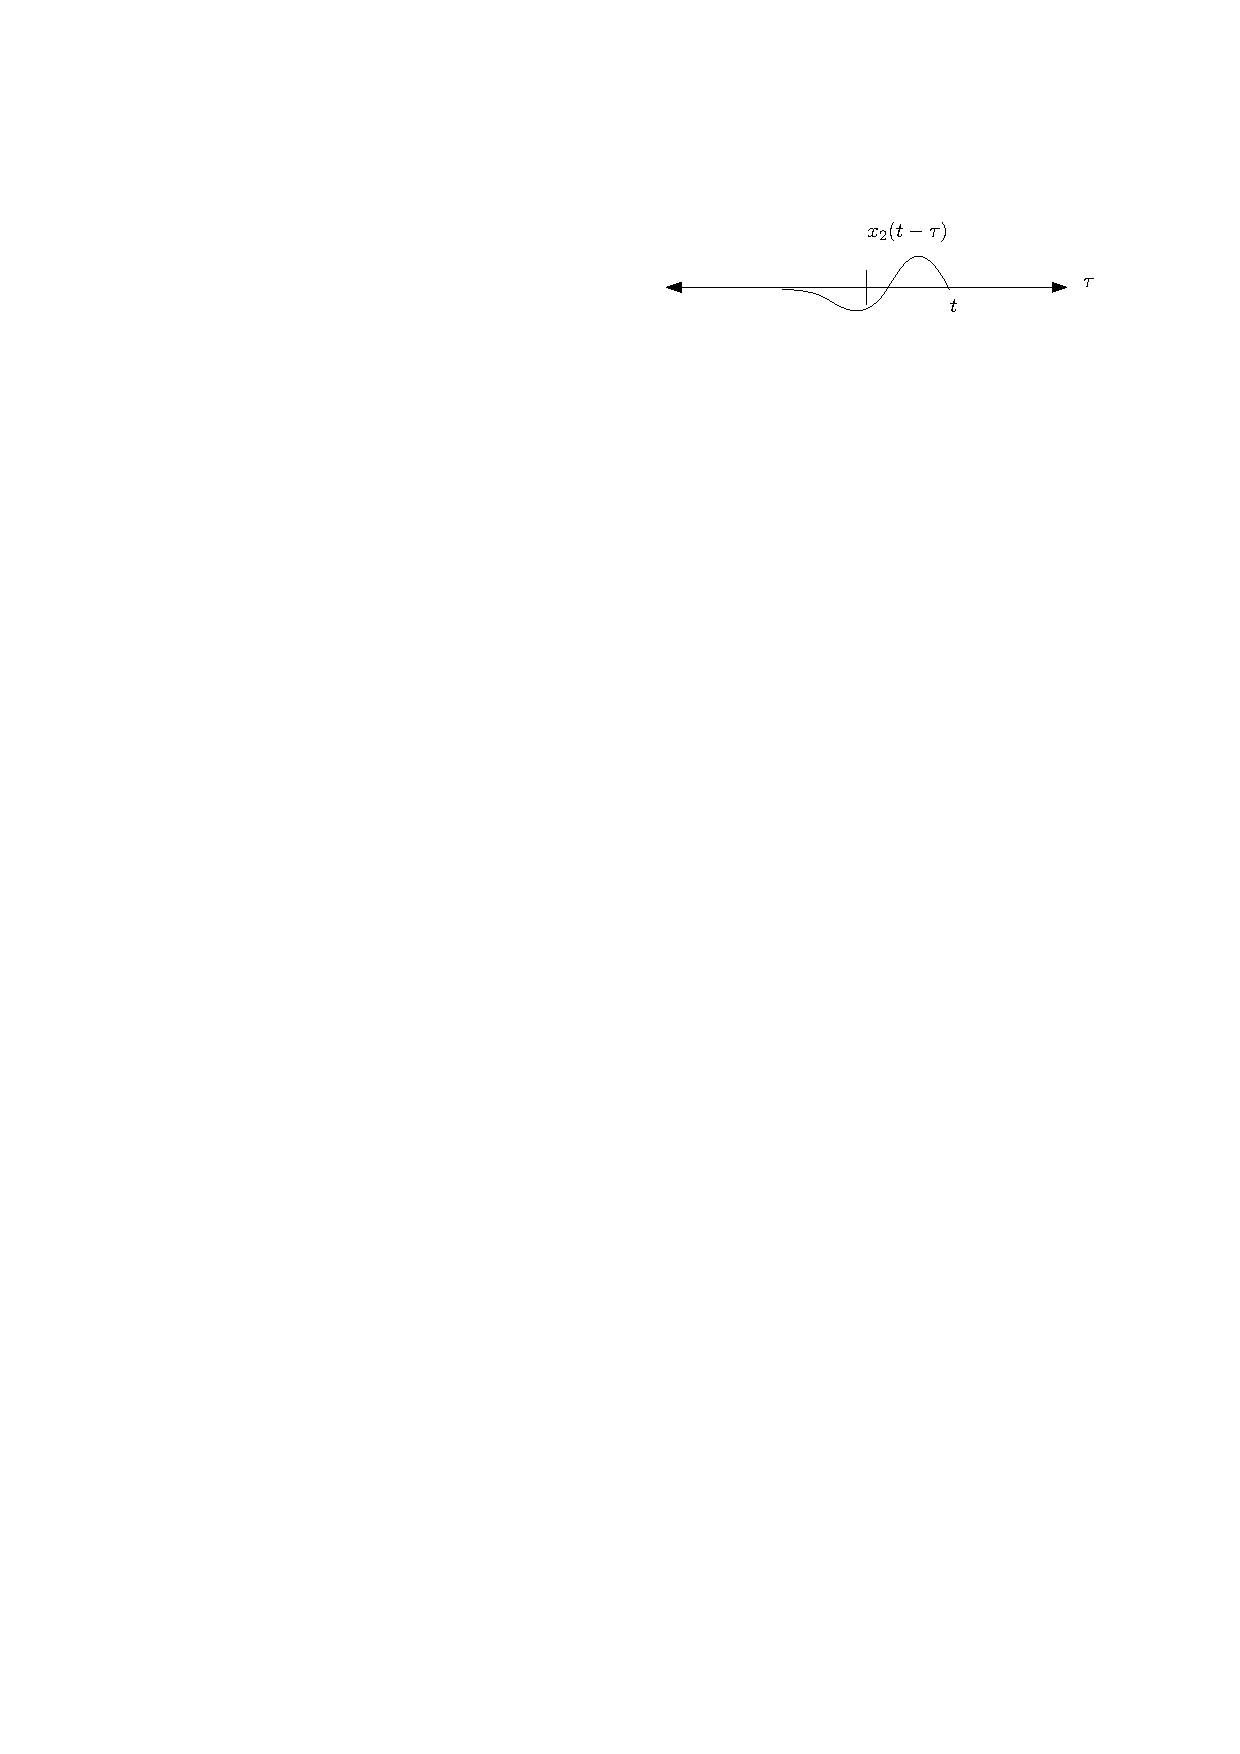
\includegraphics[scale=1]{graphics/convolution-explain3.pdf}
\end{center}
Then the integrand of convolution is the product $x_1(\tau)x_2(t-\tau)$ whose plot depends of the value of $t$. Some examples, where the individual signals are dashed and their product is in bold:
\begin{center}
  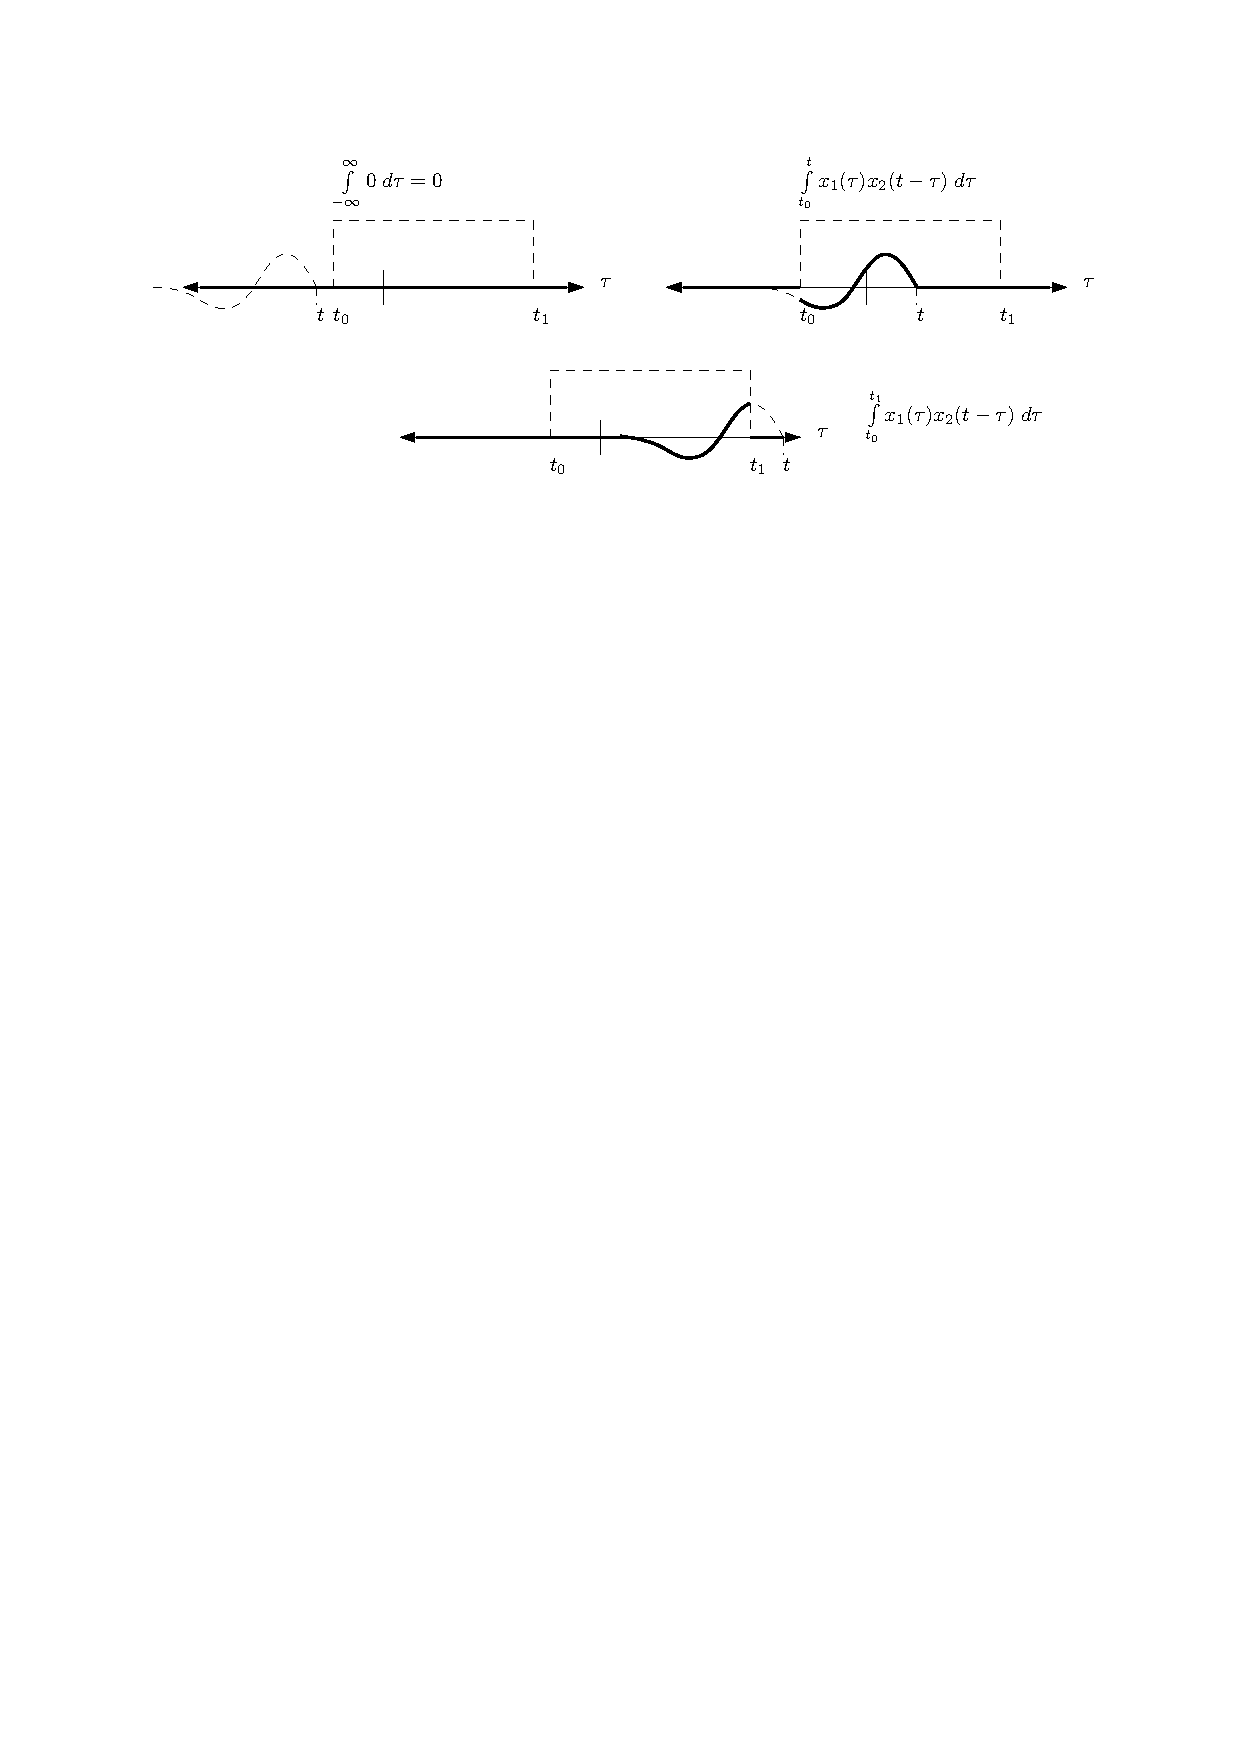
\includegraphics[scale=1]{graphics/convolution-explain4.pdf}
\end{center}
Then convolution is the total integral of the product (bold curves above) for that value of $t$. For the example above we see the integral will be zero for $t$ less than $t_0$ since the two signals do not overlap and their product is zero. For $t_0 < t < t_1$ the signals overap and the product is non-zero, and the effective bounds of integration are $[t_0,t]$. For $t > t_1$ the signals again overap and the product is non-zero, but the effective bounds of integration are $[t_0,t_1]$. 

\section{Examples of CT Convolution}

\begin{example}[$u(t) * u(t)$] Consider the convolution of two unit step functions.
  \[
  u(t) * u(t) = \int\limits_{-\infty}^{\infty} u(\tau)u(t-\tau) \; d\tau
  \]
  The product $u(\tau) u(t-\tau)$ is non-zero only when $t\geq 0$ as illustrated here
  \begin{center}
  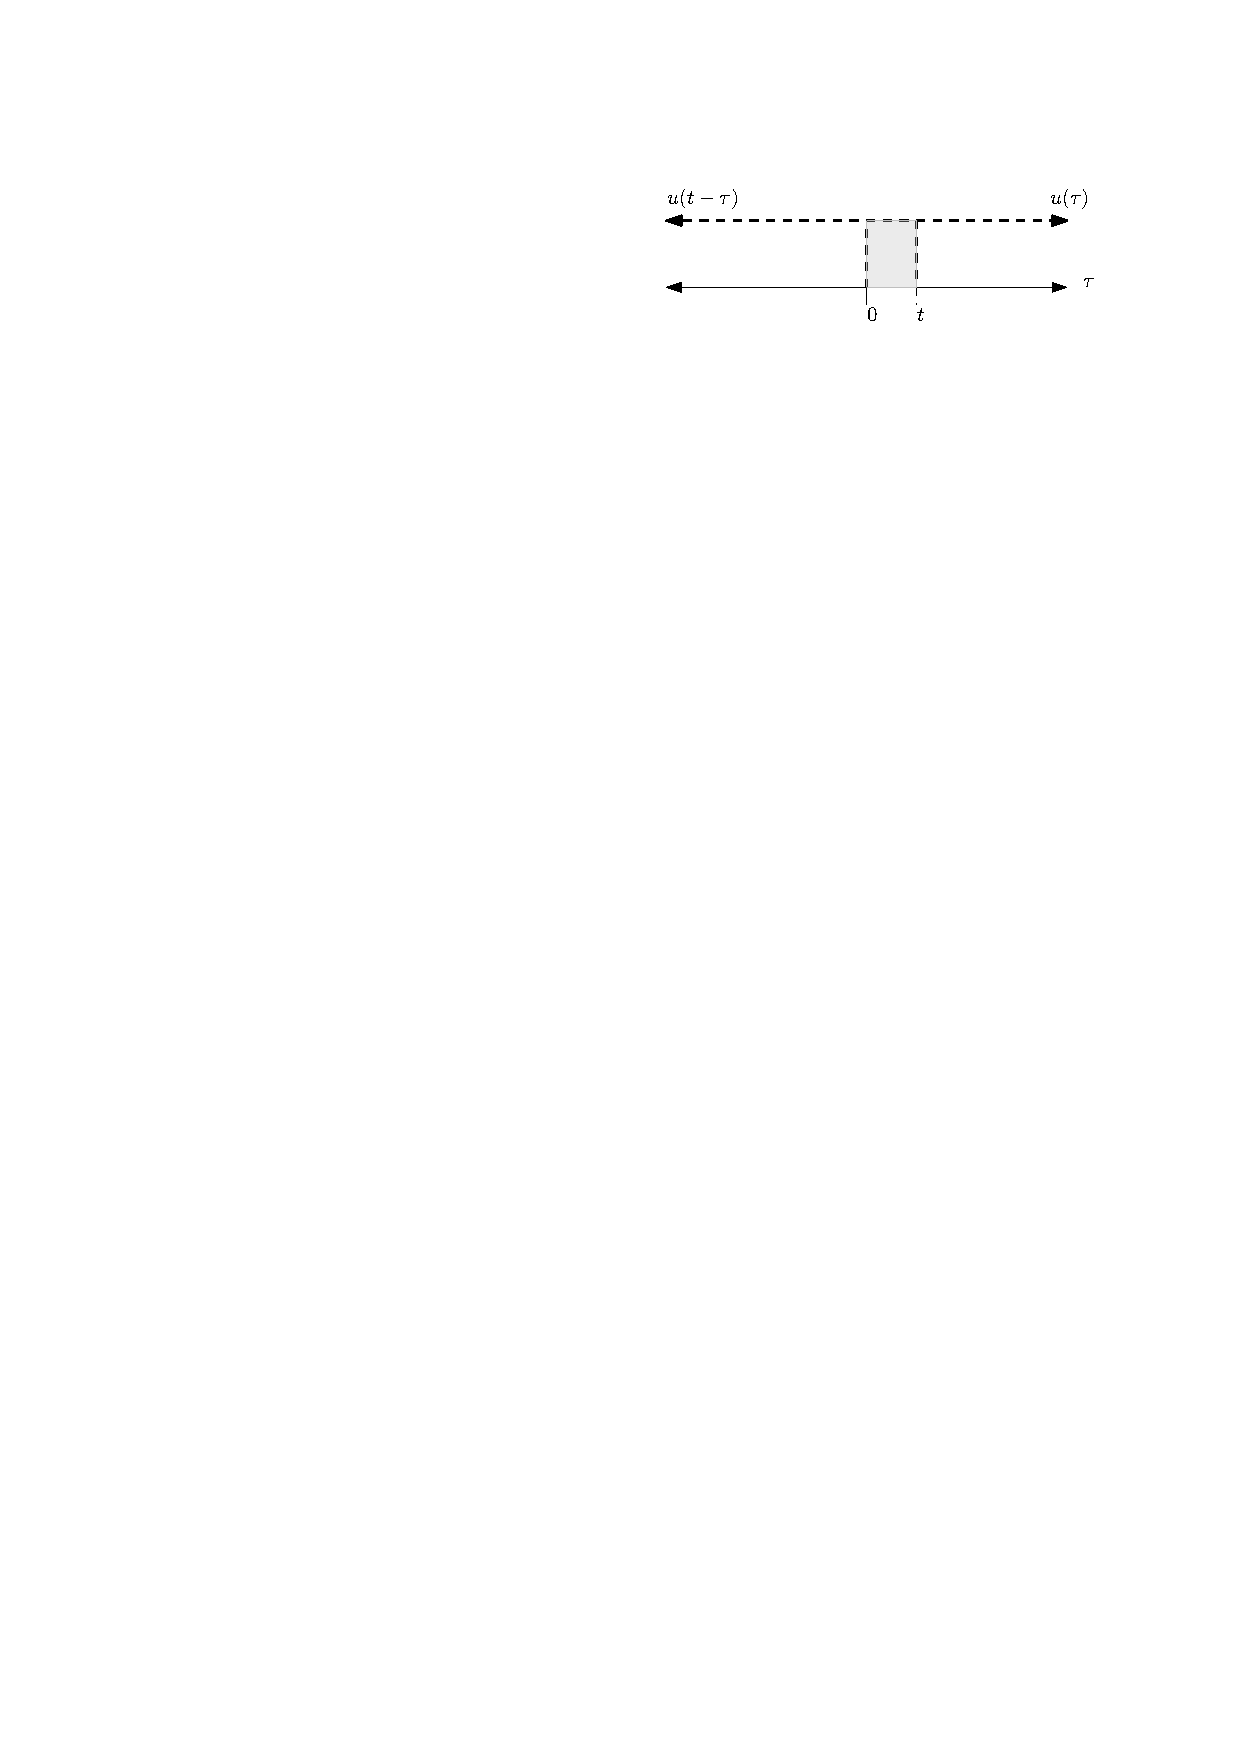
\includegraphics[scale=1]{graphics/convolution-step.pdf}
\end{center}
  The convolution integral is then the shaded area
  \[
u(t) * u(t) = \left\{ \begin{array}{lc}
  0 & t< 0\\
  \int\limits_{0}^{t} d\tau = t  & t \geq 0\\
\end{array}\right.
\]
Combining this back into a single expression gives:
\[
u(t) * u(t) = tu(t)
\]
Thus the convolution of two step signals is a ramp signal.\\$\blacksquare$
\end{example}

\begin{example}[$u(t) * e^{-at}u(t)$] Let $x_1(t) = u(t)$ and $x_2(t) = e^{-at}u(t)$ for constant $a\in\mathbb{C}$, then
  \[
u(t) * e^{-at}u(t) = \int\limits_{-\infty}^{\infty} u(\tau)e^{-a(t-\tau)}u(t-\tau) \; d\tau
\]
Similar to the previous example, the product $u(\tau) e^{-a(t-\tau)} u(t-\tau)$ is non-zero only when $t\geq 0$
  \begin{center}
  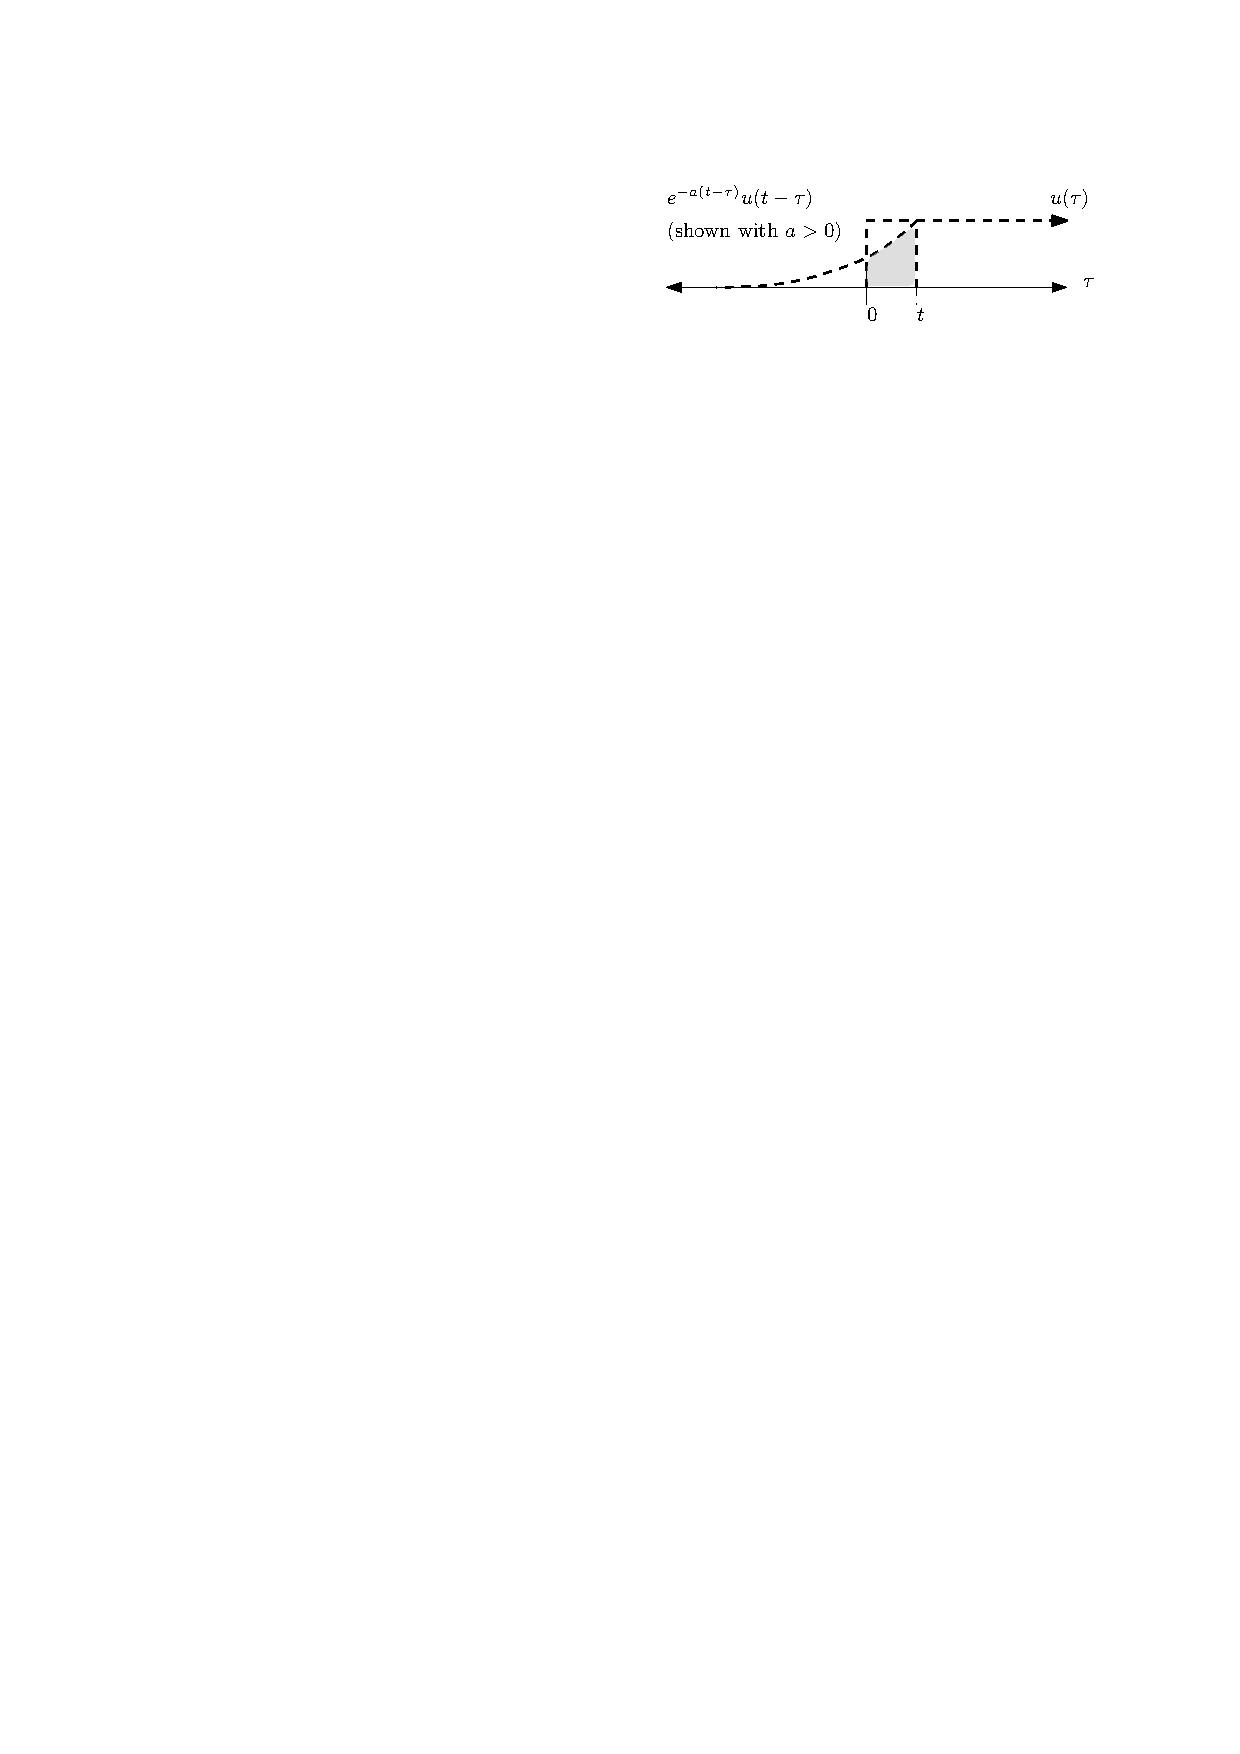
\includegraphics[scale=1]{graphics/convolution-expstep.pdf}
  \end{center}
  The convolution integral is then the shaded area
  \[
u(t) * e^{-at}u(t) = \left\{ \begin{array}{lc}
  0 & t< 0\\
  \int\limits_{0}^{t} e^{-a(t-\tau)} d\tau = \frac{1-e^{-at}}{a}  & t \geq 0\\
\end{array}\right.
\]
Combining this back into a single expression gives:
\[
u(t) * e^{-at}u(t) = \frac{1-e^{-at}}{a}u(t)
\]
$\blacksquare$
\end{example}

\begin{example}[Convolution with a delta function] Let $x_1(t) = \delta(t)$ and $x_2(t)$ be an arbitrary signal. Then
  \[
  \delta(t) * x_2(t) = \int\limits_{-\infty}^{\infty} \delta(\tau)x_2(t-\tau) \; d\tau
  \]
  By the sifting property of the delta function this evaluates to
  \[
  \delta(t) * x_2(t) = x_2(t)
  \]
  or in other words convolution with a delta function just results in the signal it was convolved with. That is it acts like the identity function, with respect to convolution.\\
  $\blacksquare$
\end{example}

The following table lists several convolution results.

\begin{center}
  Short Table of Representative Convolution Integrals
  \vspace{1em}
  
\bgroup
\def\arraystretch{2}
\setlength\tabcolsep{2em}
\begin{tabular}{|c|c|c|}
  \hline
  $x_1(t)$ & $x_2(t)$ & $x_1(t) * x_2(t)$\\
  \hline
  \hline
  $e^{a t}u(t)$ & $u(t)$ & $\frac{1-e^{a t}}{-a}u(t)$\\
  $u(t)$ & $u(t)$ & $tu(t)$\\
  $e^{a_1 t}u(t)$ & $e^{a_2 t}u(t)$ & $\frac{e^{a_1 t}-e^{a_2 t}}{a_1 - a_2}u(t)$ for $a_1 \neq a_2$\\
  $e^{a t}u(t)$ & $e^{a t}u(t)$ & $te^{a t}u(t)$\\
  $te^{a_1 t}u(t)$ & $e^{a_2 t}u(t)$ & $\frac{e^{a_2 t}-e^{a_1 t} + (a_1-a_2)te^{a_1 t}}{(a_1 - a_2)^2}u(t)$ for $a_1 \neq a_2$\\
  $e^{a_1 t}\cos(\beta t + \theta)u(t)$ & $e^{a_2 t}u(t)$ & $\frac{\cos(\theta - \phi)e^{a_2 t} - e^{a_1 t}\cos(\beta t + \theta - \phi)}{\sqrt{(a_1 + a_2)^2 + \beta^2}}u(t)$\\
  & & $\phi = \arctan\left( \frac{-\beta}{a_1 + a_2}\right)$\\
\hline                       
\end{tabular}
\egroup

\end{center}

\section{Properties of CT Convolution}
There are several useful properties of convolution. We do not prove these here, but it is not terribly difficult to do so. Given signals $x_1(t)$, $x_2(t)$, and $x_3(t)$:

\begin{description}
\item [Communative Property] The ordering of the signals does not matter.
  \[
x_1(t) * x_2(t) = x_2(t) * x_1(t)
  \]
\item [Distributive Propery] Convolution is distributed over addition.
  \[
  x_1(t) * \left[x_2(t) + x_3(t)\right] = \left[x_1(t) * x_2(t) \right] + \left[x_1(t) * x_3(t) \right] 
  \]
\item [Associative Property] The order of convolution does not matter.
    \[
  x_1(t) * \left[x_2(t) * x_3(t)\right] = \left[x_1(t) * x_2(t) \right] * x_3(t) 
  \]
\item [Time Shift] Given $x_3(t) = x_1(t) * x_2(t)$ then for time shifts $\tau_1, \tau_2 \in \mathbb{R}$
  \[
  x_1(t-\tau_1) * x_2(t-\tau_2) = x_3(t-\tau_1 - \tau_2)
  \]
\item [Multiplicative Scaling] Given $x_3(t) = x_1(t) * x_2(t)$ then for constants $a,b \in \mathbb{C}$
  \[
  \left[a\, x_1(t)\right] * \left[b\, x_2(t)\right] = a\, b\, x_3(t)
  \]
\end{description}

These properties can be used in combination with a table like that above to compute the convolution of a wide variety of signals without evaluating the integrals.

\begin{example} Here is a simple example. Let $x_1(t) = e^tu(t)$ and $x_2(t) = 2\delta(t) + 5e^{-3t}u(t)$.
  \[
  x_1(t) * x_2(t) =  e^tu(t) * \left[2\delta(t) + 5e^{-3t}u(t)\right] 
  \]
  Using the distributive property
  \[
  x_1(t) * x_2(t) =  2\left[\delta(t) * e^tu(t)\right]  + 5\left[e^tu(t) * e^{-3t}u(t)\right]
  \]
  Using previously derived results involving the delta function and the table row 3
  \[
  x_1(t) * x_2(t) = 2 e^t\, u(t) + 5\left[ \frac{e^t-e^{-3t}}{4}\right]u(t)
  \]
  Doing some simplification gives the result
  \[
  x_1(t) * x_2(t) = \left[ \frac{13}{4}e^t-\frac{5}{4}e^{-3t}\right]u(t)
  \]
  
$\blacksquare$
\end{example}

\begin{example} Here is a more complicated example. Let $x_1(t) = 2e^{-5t}u(t-1)$ and $x_2(t) = \left(1-e^{-t}\right)u(t)$.
  \[
  x_1(t) * x_2(t) = \left[2e^{-5t}u(t-1)\right] * \left[\left(1-e^{-t}\right)u(t)\right]
  \]
  We first rewrite $e^{-5t}u(t-1)=e^{-5}e^{-5(t-1)}u(t-1) = e^{-5}e^{-5t}u(t)\Big|_{t=t-1}$ so that we can remove the time shift
  \[
  x_1(t) * x_2(t) = 2e^{-5}\left[e^{-5t}u(t)\right] * \left[\left(1-e^{-t}\right)u(t)\right]\Big|_{t=t-1}
  \]
  We now apply the distributive property
  \[
x_1(t) * x_2(t) = 2e^{-5}\left[\left(e^{-5t}u(t) * u(t)\right) - \left(e^{-5t}u(t)* e^{-t}u(t)\right)\right]\Big|_{t=t-1}
  \]
  Using the table rows 1 and 3 we get
  \[
  x_1(t) * x_2(t) = 2e^{-5}\left[\frac{1}{5}\left(1-e^{-5t}\right)u(t) + \frac{1}{4}\left(e^{-5t} - e^{-t}\right)u(t)\right]\Big|_{t=t-1}
  \]
  Combining terms we simplify to
  \[
x_1(t) * x_2(t) = 2e^{-5}\left[\frac{1}{5} - \frac{1}{4}e^{-t} + \frac{1}{20}e^{-5t} \right]u(t)\Big|_{t=t-1}
\]
Replacing the time shift gives the final result
\[
x_1(t) * x_2(t) = 2e^{-5}\left[\frac{1}{5} - \frac{1}{4}e^{-(t-1)} + \frac{1}{20}e^{-5(t-1)} \right]u(t-1)
\]
which can be cleaned up a bit more by distributing the leading term
\[
x_1(t) * x_2(t) =\left[\frac{2}{5}e^{-5} -\frac{1}{2}e^{-(t+4)} +\frac{1}{10}e^{-5t}\right]u(t-1)
\]
  
$\blacksquare$
\end{example}

